\section{Generative Adversarial Networks}
\subsection{Introduction}
So far, we have seen two generative models, autoregressive models and variational autoencoders. Both of these approaches try to model $\P(x)$; autoregressive models directly maximize the likelihood of the data:
\begin{equation*}
    p_\theta(x) = \prod_{i=1}^N p_\theta(x_i|x_1, \dots, x_{i-1})
\end{equation*}
while variational autoencoders maximize the evidence lower bound:
\begin{equation*}
    \log p_\theta(x) \geq \E_{z\sim q_\varphi(z|x)}\left[\log p_\theta(x|z)\right] - \KL\left(q_\varphi(z|x)\parallel p(z)\right)
\end{equation*}
Both of these models have their limitations; autoregressive models are slow to sample from, and variational autoencoders can have blurry samples. Generative adversarial networks (GANs) are a third approach to generative modeling that can generate high-quality samples quickly, by focusing on the problem of generating samples from a distribution instead of trying to explicitly model the distribution.

\subsection{Generator and Discriminator}
Assume that we have acces to some data samples $x_i$ drawn from a certain distribution $p_{\text{data}}$. Our goal is to draw new samples from $p_{\text{data}}$, without trying to access its values. Similarly to variational autoencoders, we assume that each sample is associated to a latent variable $z$ with a simple prior distribution $p(z)$. The idea is to learn a \emph{Generator Network} $G(z)$ that takes a latent variable $z$ as input and outputs a sample $x = G(z)$. $G$ implicitely defines a probability distribution $p_G$ over the samples $x$; we want to learn $G$ such that $p_G$ is as close as possible to $p_{\text{data}}$.

In parallel, we will train a \emph{Discriminator Network} $D$ to perform a classification task: given a sample $x$, $D(x)$ should output the probability that $x$ is a sample from $p_{\text{data}}$ rather than $p_G$. The training of $D$ is supervised: it is trained on both real samples $x_i$ and fake samples $G(z)$, of which we know the labels $0$ and $1$ respectively.
\begin{figure}[H]
    \centering
    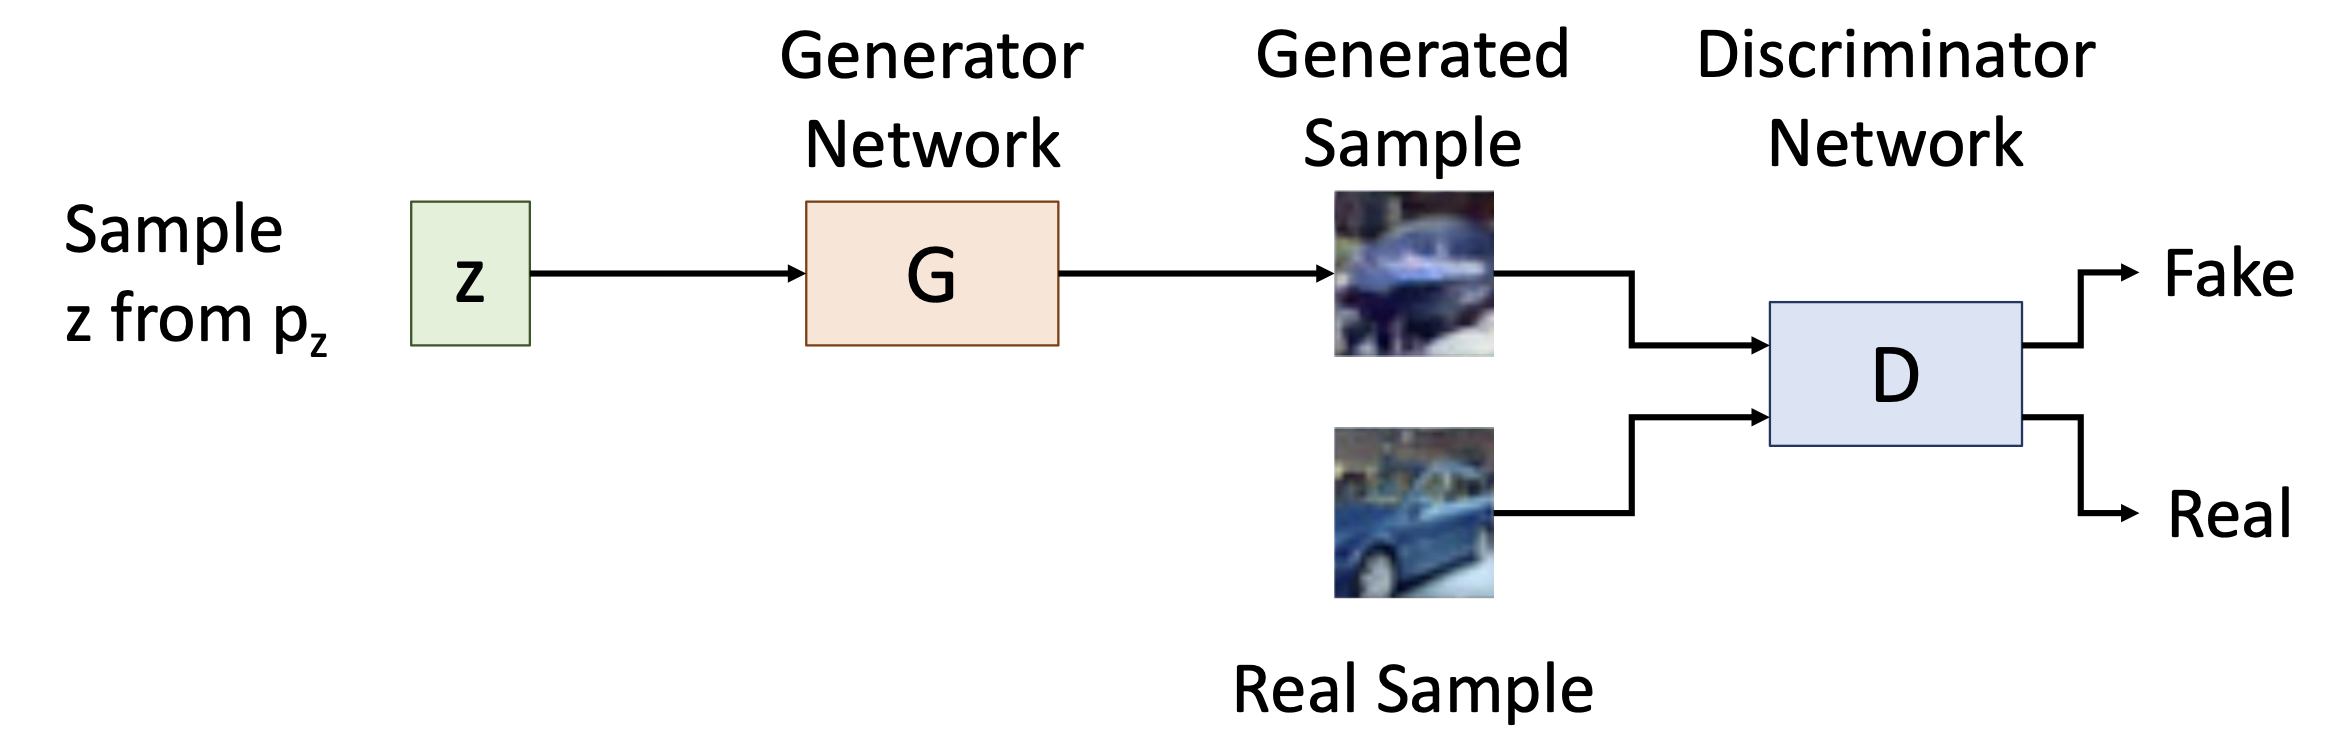
\includegraphics[width=.9\textwidth]{gans/generator-discriminator.png}
\end{figure}
We train the Generator $G$ and the Discriminator $D$ in an \emph{adversarial} manner: $G$ tries to fool $D$ by generating samples that are indistinguishable from real samples, while $D$ tries to distinguish between real and fake samples.

\subsection{Training objective}
We will jointly train the Generator $G$ and the Discriminator $D$ with a \emph{minimax game}. A first objective to optimize for is the following:
\begin{equation}
    \min_G\max_D \left(
        \E_{x\sim p_{\text{data}}}\left[\log D(x)\right] + \E_{z\sim p(z)}\left[\log\left(1-D\left(G(z)\right)\right)\right]
    \right)
\end{equation}
The Discriminator wants $D(x)=1$ for real data and $D(x)=0$ for fake data. Therefore, the first inner quantity $\E_{x\sim p_{\text{data}}}\left[\log D(x)\right]$ is the $\log$-likelihood of a real sample being classified as real, while the second inner quantity $\E_{z\sim p(z)}\left[\log\left(1-D\left(G(z)\right)\right)\right]$ is the $\log$-likelihood of a fake sample being classified as fake. The objective of the Discriminator is to maximize both these quantities, while the Generator tries to minimize them.

Let $V(G, D) = \E_{x\sim p_{\text{data}}}\left[\log D(x)\right] + \E_{z\sim p(z)}\left[\log\left(1-D\left(G(z)\right)\right)\right]$. The training loop will consist in alternating between the optimization of $D$ and $G$; for $t\in\iset{0}{T}$:
\begin{enumerate}
    \item Update $D$: \begin{equation*}D\longleftarrow D+\alpha_D\frac{\partial V}{\partial D}\end{equation*}
    \item Update $G$: \begin{equation*}G\longleftarrow G-\alpha_G\frac{\partial V}{\partial G}\end{equation*}
\end{enumerate}
Note that we are not minimizing any overall loss; the generator and the discriminator have their own loss, which depend on each other and is usually not monotonically decreasing.

In practice, at the start of training, the generator performs quite poorly while the dicriminator can easily tell apart real and fake data, making $D(G(z))$ very close to $0$. This usually leads to a vanishing gradient for $G$. To avoid this, instead of training $G$ to minimize $\log\left(1-D(G(z))\right)$, we train it to minimize $-\log D(G(z))$.

\subsection{Optimality}


\newpage